\section{Model, Assumptions and Problem Formulation}
\label{sec:problemformulation}

% Background and problem model
\subsection{Model and Assumptions}
\label{subsec:model}

% Background
% Multiband variation
Wireless propagation refers to the signal loss characteristics when wireless signals 
are transmitted through the wireless medium. The strength of the received signal depends on 
both the line-of-sight path (or lack thereof) and multiple other paths that result from reflection, 
diffraction, and scattering from obstacles~\cite{andersen1995propagation}. The widely-used Friis
equation characterizes the received signal power $P_r$ in terms of transmit power $P_t$, transmitter 
gain $G_t$, receiver gain $G_r$, wavelength $\lambda$ of the carrier frequency, distance $R$ from 
transmitter to receiver, and path loss exponent $n$ according to~\cite{friis}:
\begin{equation}
\label{eq:friis}
P_r=P_t+G_t+G_r+10n \log_{10}\left( \frac{\lambda}{4\pi R}\right)
\end{equation}
Here, $n$ varies according to the aforementioned environmental 
factors with a value ranging from two to five in typical outdoor 
settings~\cite{rappaport}.
% Tell the propagation of white space is much larger than wifi
Thus, the channels of white space bands propagates further than the channels of the WiFi bands in 
free space under the same RSSI threshold, transceiver settings~\ref{eq:friis}. 
% White spcae is good out resource to improve the service of Wifi cell
The propagation range of white space channels could be many times of WiFi channels, for instance, 
450 MHz channels has more than 12 times propagation range as 5 GHz channels. The larger propagation 
of white space channels make it possible to assist a WiFi mesh with few white space channels. 
% Power saving


\begin{figure}
\vspace{-0.0in}
\centering
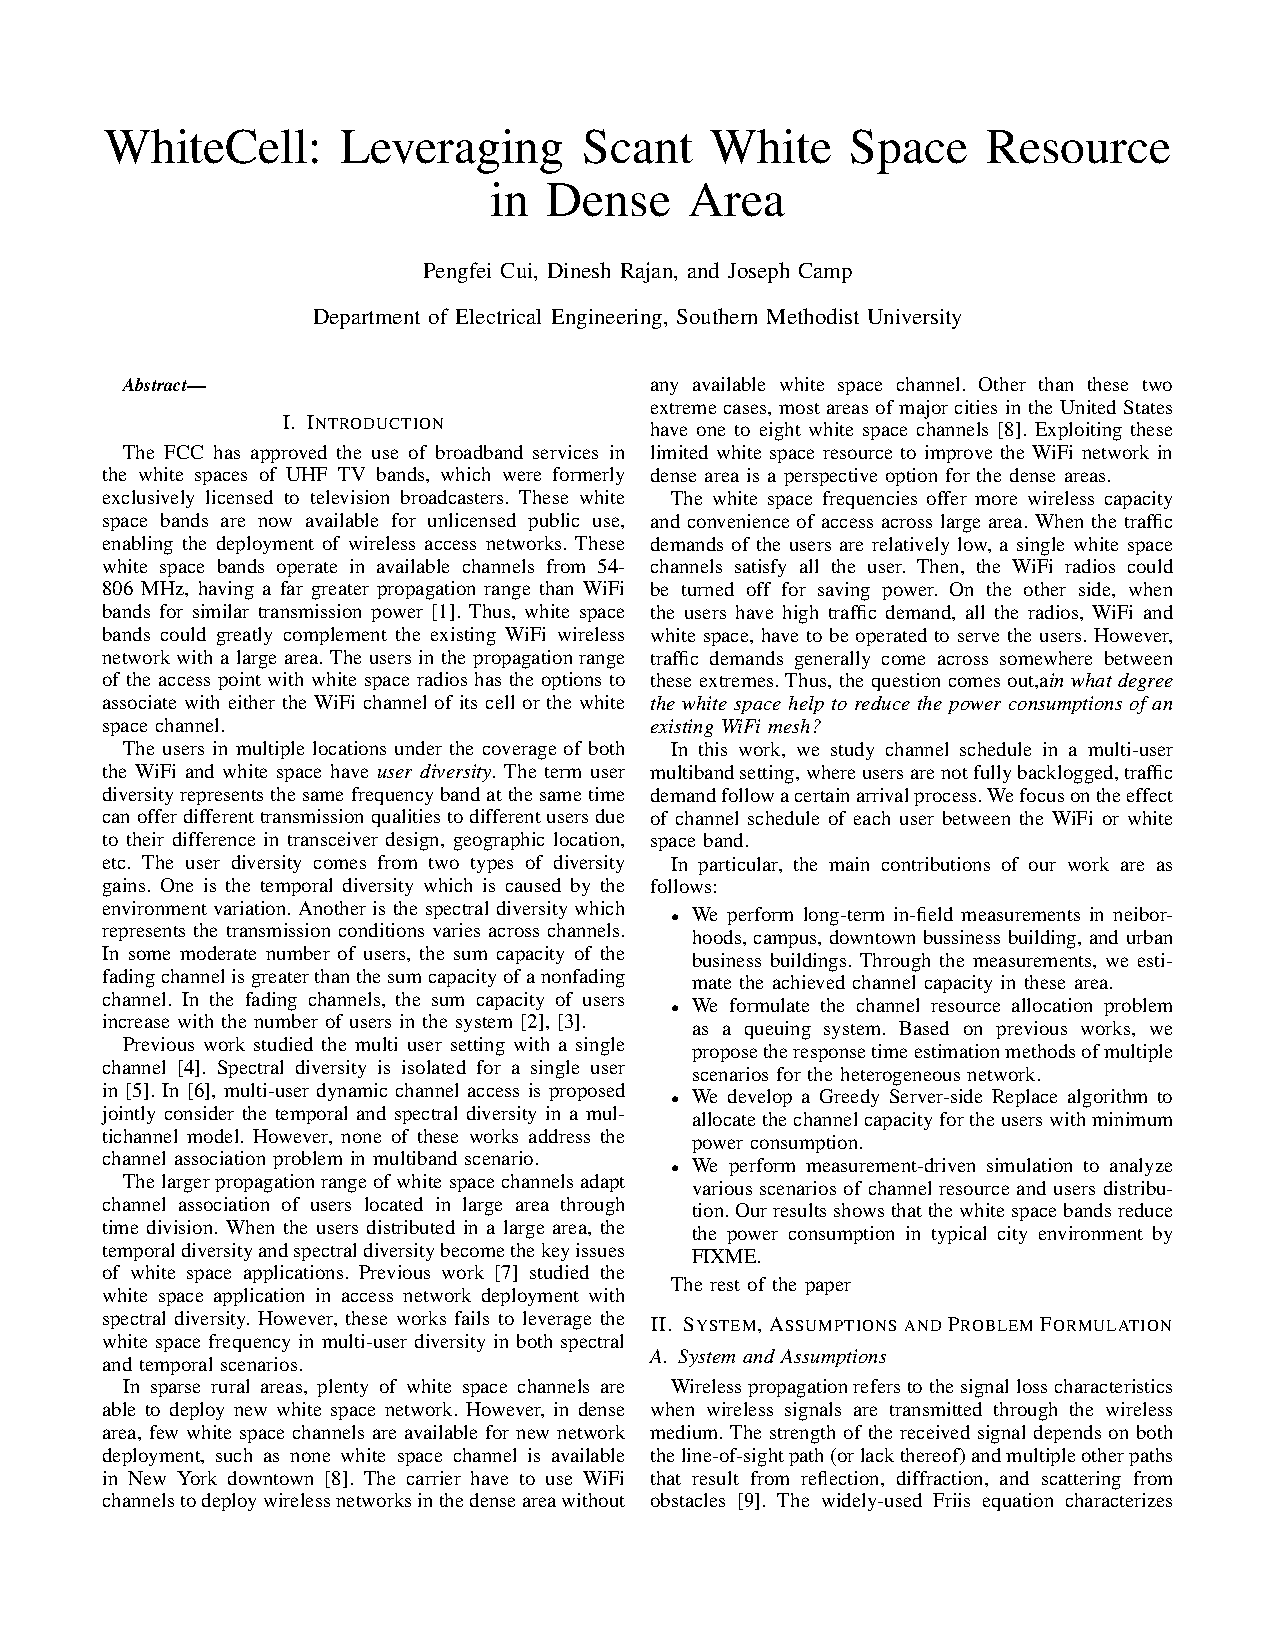
\includegraphics[width=74mm]{figures/whitecell}
\vspace{-0.1in}
\caption{White Space Model in Dense Area}
\label{fig:systemmodel}
\vspace{-0.1in}
\end{figure}


% Give the model and assumption
% B channel; N user; M AP;
Given a WiFi mesh wireless system with $M$ access points and $N$ users as shown in Fig.~\ref{fig:systemmodel}. 
The users are scheduled with the access point on the single channel $f \in F_M$ located in its own mesh. We consider $F_w$ 
new white space radios is installed on one of the access points to assistant the existing WiFi network. The 
capacity of each radio $C$ is a equally restrict number of all the channels. For each user, it has $1+F_w$ 
channels to be scheduled, the previous WiFi channels and the new white space channels. 
Then the $N$ users has the options to schedule either WiFi or the new white space channels. 
The channel capacity of the scheduled channels between the access points and users is 
noted as a matrix in Eq.~\ref{eq:usercapacity}
\begin{equation}
\label{eq:usercapacity}
H_{i,j}^f(t)= f(\lambda,t),i \in M, j\in N, f \in (1+F_w) 
\end{equation} 
$\lambda$ represents the in-field measured historical data and dynamic sensing information.
We use a context-aware method to estimate the $j$ user capacity $H_{i,j}^f(t)$ to an access point 
$i$ on channel $f$. We assume the users from the same mesh cell are in a single interference 
domain, so these users have to apply a time division for the WiFi channel assigned for this cell. 
Only one user of the system could occupy a single channel during a time slot. Considering the 
limited number of white space channels in dense area and the fact spatial reuse of white space 
will make the problem considerably more challenging, we will remains an interesting direction 
of future research. 

In this system, the channel capacity $H_{i,j}^f(t)$ is from the SNR according to Friis model and in-field 
measurements. We consider discrete time with a suitably chosen small time unit. 
%One user can only associate 
%with a single channel during a time slot to avoid heavy interference. 
Users scheduled with the same channel will share the time unit. We will assume the channel capacity of 
the channel schedule keep flat during the time unit. 
Each user faces $F_w+1$ options: schedule with the assigned WiFi channel or one of the white space 
channels. We assume the switching time is negligible. The traffic demand arrive at a user as a Poisson process, 
with the vector noted as $\bm{D} = [D_1,D_2,...D_N]$ and the sum rate $D = \sum\limits_{i=1}^N D_i$.  The rate $D$ 
is the aggregate rate of data generated from all users. 
%The served traffic flow $\Gamma$ represents the traffic 
%delivered to the access points through the wireless channels.



% Buffer and tolerance time
Each user has $B$ buffer store the traffic demand. As discussed in ~\cite{niida2010user}, the tolerance 
time of traffic varies from text information, voice information. To address the user tolerance time, we 
have the waiting time constraint $\mu_j,j\in N$ based on the users traffic demand types.  
% Buffer assumptions
Through this waiting time constraint, the waiting time of a user is limited in a certain time window, 
which means the traffic of a user will be served during the tolerance time to satisfy the QoS requirements.
We assume the buffer $B$ is large enough to store the data during the tolerance time.
%We define the payoff function according to the waiting time of user's traffic and traffic types in Eq.\ref{eq:payoff}. 
%To address the user tolerance time, we build the payoff functions based on the users traffic demand and the buffered time of the 
%traffic demand to process the channel schedule. Through this payoff function, the waiting time of a user is limited in 
%a certain time window, which means a user will be served at least once to satisfy the QoS requirements.
%We define the payoff function according to the waiting time of user's traffic and traffic types in Eq.\ref{eq:payoff}. 
%
%% Payoff B, benefit
%\begin{equation}
%\label{eq:payoff}
%\xi=\sum \alpha^{t_d}\cdot T
%\end{equation}
%%$\alpha$ is a parameter represents the traffic types. 
%To represents the variation, we define the $\alpha \ge 1$ to represent the tolerance of traffic
%type to make an individual user stay in the tolerance time. 
%$t_d$ is the time the user has waited for the traffic in the queue. Through the definition, the traffic could be 
%scheduled according to the traffic type and the waiting time. 
%According the the payoff function, the expected benefit of a served beam schedule could be calculated through the BBS framework.
%With BBS, the time efficient for the system is increased and the satisfaction of users and power efficient.




\subsection{Problem Formulation}
\label{subsec:problem}


The previous problem is formulated as a discrete-time queuing system as shown in Fig.~\ref{fig:flowconfig}.
We list each single channel for the users as a server.
Table.~\ref{tab:notation} summarizes the notation used in this work.
The system has $N$ queues and $F_M+F_w$ servers connecting by time-varying channels $H^*(N,F_M+F_w)$.



\begin{table}[htbp]
\begin{center}% used the environment to augment the vertical space
% between the caption and the table
\begin{tabular}{l l p{10cm} }
\toprule
$t$ & Time slot\\
$N$ & Set of users\\
$M$ & Set of WiFi cells\\
$H_{ij}^f$ & Measurement based Capacity between AP i and user j on channel f\\
$F_{m}$ & WiFi Channels in the cells\\
$F_{w}$ & Set of White Space Channels\\
$A(t)$ & User access channel schedule\\
$C$ & Clean Radio Capacity\\
$D$ & User Demand\\
$R$ & Operating Radio\\
$\zeta$ & In-Field Measurements\\
$W$ & User Tolerance time window \\
$\mu$ & Channel capacity assigned for a cell \\
$P_s$ & Standby Power Consumption \\
$P_t$ & Transmission Power Consumption \\
%$R_{i}$ & $\triangleq$ & Revenue at store $i$\\
%$i$ & $\triangleq$ & index value for store locations\\
%${T}_{c}$ & $\triangleq$ & A very long description of this specific variable and is needed in the research and looks good when wrapped and aligned to the left.\\
%$TC$ & $\triangleq$ & Total overall cost(\$)\\  
%\multicolumn{3}{c}{}\\
%\multicolumn{3}{c}{\underline{Decision Variables}}\\
%\multicolumn{3}{c}{}\\
%$y_f$ & $=$ & \(\left\{\begin{array}{rl}
%1,  & \text{if Supplier located at site $f$ is open} \\
%0,  & \text{otherwise} \end{array} \right.\)\\
\bottomrule
\end{tabular}
\end{center}
\caption{Table of Notations}
\label{tab:notation}
\vspace{-0.3in}
\end{table}





\begin{figure}
\vspace{-0.0in}
\centering
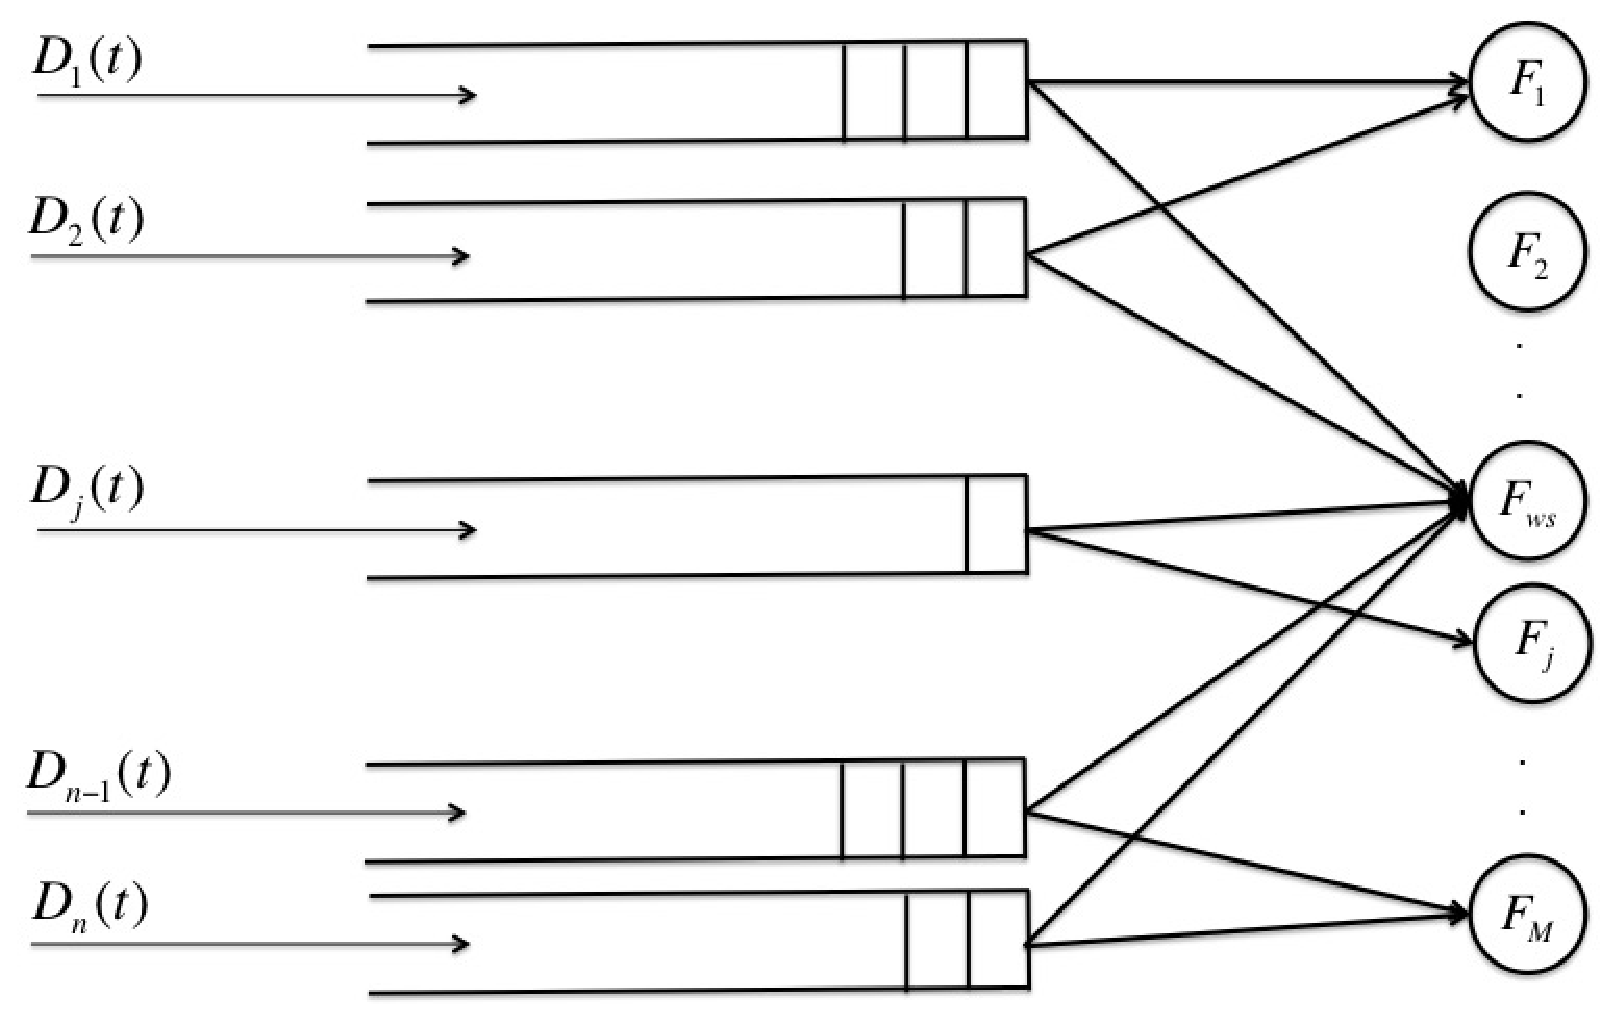
\includegraphics[width=84mm]{figures/flowconfig}
\vspace{-0.1in}
\caption{System Model}
\label{fig:flowconfig}
\vspace{-0.1in}
\end{figure}


In this system, during a time unit, the users need to schedule with an access point on a channel. 
Let matrix \{$A_{i,j}(t),i\in (F_M+F_w), j\in N$\} denote a schedule meets the performance constraints 
will be discussed later.
%where $A_{i,j}^b = 1$ denotes user $j$ is scheduled with access point $i$ on channel $b$.
\begin{equation}
\label{eq:associate_def}
 A_{i,j}(t) = \left\{ 
	  \begin{array}{l l}
	    1   &  if\ D_{j\in N},\ is\ scheduled\ with\ channel\ j \in (F_M+F_w) \\
		0 &  Otherwise
			    \end{array} \right.
\end{equation}



%We assume one user can only associate with a single access point on a single channel in Eq.~\ref{eq:associate}
%\begin{equation}
%\label{eq:associate}
%\sum\limits_{i=1}^{M+B} A_{i,j} \le 1
%\end{equation}
%We now analyze the traffic with the objective of maximizing the served traffic flow over the channel 
%association.



With a schedule $A$, the served traffic flow of a user is the minimize value of the queue when then have 
enough capacity, or the remaining capacity as shown in Eq.\ref{eq:effectiverate}


\begin{equation}
\label{eq:effectiverate}
 \gamma_j(t) = \left\{ 
	  \begin{array}{l l}
	     \min\limits_{j\in N}(Q_j(t),\sum\limits_{i=1}^{F_M+F_w} A_{i,j}(t) \cdot H_{i,j}(t))   &  \sum\limits_{j=1}^N \gamma_j(t) \cdot A_{i,j}(t) \le C\\
		0 &  \sum\limits_{j=1}^N \gamma_j(t) \cdot A_{i,j}(t) > C
			    \end{array} \right.
\end{equation}


The individual queues $Q_j(t),j\in N$ at the end of the time slot $t$ is represented as Eq.~\ref{eq:userqueue}:
\begin{equation}
\label{eq:userqueue}
%Q_j(t) = Q_j(t-1)+D_j(t)-\min{\{\sum\limits_{i=1}^{(F_m+F_w)} H_{i,j}(t)\cdot A_{i,j}(t),Q_j(t-1)}\}
Q_j(t) = Q_j(t-1)+D_j(t)- \gamma_j(t)
\end{equation}


% Waiting time constraint
The total transmission time must be smaller than the tolerance time. 
\begin{equation}
\label{eq:timelimit}
\sum\limits_{t^*}^{t^*+\mu_j}\gamma_j(t^*) \ge Q(t^*)+D(t^*), j\in N
\end{equation}
$\mu_j$ is the tolerance time of each user.

% Radio representation
The operated radios $R_i$ in the system is chosen from the WiFi radios $F_M$ and the white space radios $F_w$. 
If the a radio $R_i$ is chosen, $R_i = 1$, otherwise $R_i = 0$, as shown in Eq.~\ref{eq:radio}
\begin{equation}
\label{eq:radio}
 R_i(t) = \left\{ 
	  \begin{array}{l l}
	    1   &  \sum\limits_{j=1}^N A_{i,j}(t) \ge 1\\
		0 &  Otherwise
			    \end{array} \right.
\end{equation}


The goal is to minimize the channel resource required as shown in Eq.~\ref{eq:objective}:
\begin{equation}
\label{eq:objective}
\xi = \min{\{\sum\limits_{t}^{t+T}\sum\limits_{i}^{(F_M+F_w)} R_{i}}(t)\}
\end{equation}
$T$ noted the duration time slots to reduce the resource utilization.


% Here


% Extreme cases
%$A^*$ is the global association of the wireless system to achieve the maximize served traffic flow $\Gamma*$.
%When the traffic demand of the users is small, $D \ll C$, the users are free to choose any channel for association. 
%However, as the traffic demand increase, it becomes difficult to associate the channels to the users and access points.
%A particular user has to know how the others associate with channels in prior to get the optimal association.


% Reduce the radio/server/channel resource



% New section feasibility, and Max flow formulation

%The model could be formulated as a {\it Max-Flow} problem~\cite{networkoptimization}. The question is 
%looking for a feasible flow $\Gamma$ under the constraints of channel capacity $H$ and traffic demand $D$. 
%The lower bound of flow is $0$, the upper bound of a single flow from the accss point $i$ to user $j$ is 
%the measurements based $H_{i,j}^b$.
%Thus, $\gamma_j \le \sum\limits_{i\in M} \sum\limits_{b \in B} H_{i,j}^b\cdot A_{i,j}^b$. The max-flow model 
%of the problem is feasible. 

